\chapter{Background}

\section{Introduction to Fuzzing}
Fuzzing, or fuzz testing, is a software testing technique that includes feeding a huge amount of random data into the system, called SUT (System Under Test), to find unprecedented responses and reveal major programming errors, along with key security vulnerabilities. The primary objective of fuzzing is to identify vulnerabilities such as buffer overflows, memory leaks, and other security weaknesses that can be exploited by attackers.
\\The success of fuzzing is based on its capabilities for automatic test case generation and for focusing its attention on portions of programs that otherwise would not have been tested by other more traditional testing technique.
\\Indeed, it is particularly effective for applications with complex input grammars, where manual test case creation would be impracticable.

\subsection{Types of Fuzzing Techniques}
Fuzzing methodologies vary, and there exist a lot for different applications and purposes:

\begin{itemize}
    \item \textbf{Black-box Fuzzing}: This is a technique of generating inputs without prior knowledge of the internal structure of an application. It is easy to deploy but often less efficient as there is no internal feedback.
    
    \item \textbf{White-box Fuzzing}: This is one of those techniques that rely heavily on source code intuition, such as control flow and data flow, to provide maximum code coverage with test case generation. The approach often employs some sort of complex static and dynamic analysis methodologies.
    
    \item \textbf{Grey-box Fuzzing}: It's a strategy that combines the various merits of black-box and white-box fuzzing. It brings in partial knowledge about internal application details, and code coverage feedback guiding the generation of inputs. It balances simplicity with effectiveness, and an example might be the family of tools called AFL (American Fuzzy Lop).
    
    \item \textbf{Mutation-based Fuzzing}: This generates new inputs through random mutations of existing inputs. It requires no knowledge about the structure of the inputs but is often a lot weaker compared with other generations for applications requiring highly structured inputs.
    
    \item \textbf{Generation-based Fuzzing}: This builds the inputs from scratch, based on a formal characterization of the input format, grammar or protocol specification. It has proved quite effective in applications where the inputs have to be complex or systematically structured.
\end{itemize}

\section{Stateful Fuzzing: Concepts and Challenges}
\textit{Stateful fuzzing} adds state awareness to traditional fuzzing methods. Traditional fuzzing approaches treat every input individually as a test case, but stateful fuzzing considers an application's internal state and how that state might affect subsequent inputs handling. This becomes particularly critical for applications that handle complex state information, such as network servers, databases, and interactive applications.

\subsection{Understanding Stateful Applications}
Stateful applications maintain state across multiple interactions or sessions. Examples include network servers that manage connection states, authentication states, session identifiers, or other state information specific to an application. These states significantly influence the processing of inputs and the behavior of the application over time.
\\Good practices in state transition management are crucial for both security and reliability: bugs related to state transitions can lead to vulnerabilities such as unauthorized access, denial of service (DoS), or data corruption. 
\\Stateful fuzzers attempt to model and explore these state transitions by generating input sequences that mimic valid usage scenarios while concurrently monitoring state changes to ensure comprehensive coverage of all possible transitions. To better understand this concept, consider a simple state model shown in Figure \ref{fig:simplestatemodel}.

\begin{figure}[h]
    \centering
    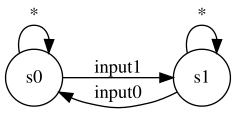
\includegraphics[width=0.5\textwidth]{Images/simplestatemodel.png}
    \caption{A simple state model illustrating state transitions in a stateful application}
    \label{fig:simplestatemodel}
\end{figure}


\subsection{Key Techniques in Stateful Fuzzing}
Stateful fuzzing involves several advanced techniques that distinguish it from traditional fuzzing approaches:

\begin{itemize}
    \item \textbf{State Modeling}: The process of building a model representing an application state machine by reverse engineering source code, observing real interactions, or guide test case generation in conjunction with machine learning techniques.
    
    \item \textbf{State Tracking}: This involves tracking the state of the application across successive inputs; indeed, tracking of network traffic, system calls, or internal state variables.
    
    \item \textbf{Feedback Mechanisms}: With feedback mechanisms, one can prioritize those test cases that tend to explore new states or code paths; hence, the general efficiency of fuzzing can be improved.
    
    \item \textbf{Sequence Generation}: It is the need to generate input sequences to properly model actual use, since the findings of vulnerabilities often depend on specific sequences or state transitions.
    
    \item \textbf{Learning-Based Approaches}: Certain fuzzers utilize machine learning or heuristic methodologies to dynamically ascertain the structural configuration of the application's state machine, thereby enabling the fuzzer to adjust and enhance its efficacy progressively.
\end{itemize}

\subsection{Challenges in Stateful Fuzzing}
Successfully performing testing is fraught with several challenges in stateful fuzzing:

\begin{itemize}
    \item \textbf{State Explosion}:As in real life, an application itself may have a number of possible states, and with more states, a risk for exponential growth in process complexity increases. In this case, state abstraction, pruning, or prioritization counters the \textit{state explosion} in an essential way.
    
    \item \textbf{Protocol Complexity}: Generating meaningful input sequences can involve deep knowledge of complex protocols or state machines. This often includes much domain-specific knowledge or even advanced algorithms.
    
    \item \textbf{Performance Overhead}: To date, state tracking performed by the application and input sequence generation can cause significant computational costs, hence slowing down the fuzzing process.

    \item \textbf{Handling Non-Deterministic Behavior}: The nondeterministic behavior of stateful applications often results from concurrency, differences in external inputs, or even timing variations. These factors therefore make the reproduction of bugs and receiving consistent fuzzing results usually difficult.

\end{itemize}

\section{Lighttpd: A Case Study for Stateful Fuzzing}
\textit{Lighttpd} is an open-source web server optimized for performance with very low memory usage. It is designed to handle huge volumes of parallel connections with minimal overhead, making it particularly useful on systems with limited resources or those requiring a high degree of concurrency. Its modular design and support for advanced web protocols make it a popular choice for embedded systems, cloud computing platforms, and high-traffic websites.

\subsection{Overview of Lighttpd Architecture}
Lighttpd operates on an event-driven architecture, which enables it to serve many requests concurrently. An asynchronous I/O framework is employed to minimize overhead in network connections, allowing the server to scale efficiently under varying workloads. The key features of Lighttpd include:

\begin{itemize}
    \item \textbf{Modular Design}: Provides a series of modules for implementing functions like URL rewriting, HTTP compression, SSL/TLS, and WebSockets. The modular design allows for customization based on specific needs.
    
    \item \textbf{Protocol Support}: Out of the box, it supports HTTP/1.1, HTTPS, FastCGI, SCGI, and HTTP/2, making it suitable for a wide range of web applications and services.
    
    \item \textbf{Security Attributes}: Advanced integrated security features include TLS/SSL encryption, prevention of denial-of-service attacks, and multiple authentication options.
\end{itemize}

\subsection{Relevance of Lighttpd for Fuzzing}

Lighttpd is an important target for stateful fuzzing due to its complex state management and the potential vulnerabilities that can emerge from improper state handling. As a web server commonly used behind various internet applications, Lighttpd needs to manage multiple simultaneous connections and support multiple network protocols. These characteristics make it a suitable candidate for evaluating stateful fuzzing techniques. By applying stateful fuzzing to Lighttpd, researchers can assess the capability of these tools to discover vulnerabilities that traditional fuzzing methods might miss.

\section{Fuzzers Overview: AFLNet, ChatAFL, and Fallaway}

For this thesis, three stateful fuzzers—AFLNet, ChatAFL, and Fallaway—will be benchmarked over Lighttpd.

\subsection{AFLNet}
\textit{AFLNet} \cite{AFLNet} is a greybox fuzzer for protocol implementations. Unlike existing protocol fuzzers, it takes a mutational approach and uses statefeedback besides code-coverage feedback in order to guide the fuzzing process. AFLNet is seeded with a corpus of recorded message exchanges between the server and an actual client. No protocol specification or message grammars are required. It acts like a client, replaying variants of the original sequence of messages ever sent to the server, retaining only the variants which managed to increase the coverage of either code or state space. The response codes supplied by the server are utilised by AFLNet for server states that a message sequence manages to exercise. From this feedback, AFLNet identifies progressive regions in the state space and systematically steers towards such regions. 



\subsection{ChatAFL}
\textit{ChatAFL} \cite{chatafl} is a large language model-guided protocol fuzzer. It is based on AFLNet but integrates three concrete components. First, the fuzzer uses the LLM to extract a machine-readable grammar for a protocol that is used for structure-aware mutation. Second, the fuzzer uses the LLM to increase the diversity of messages in the recorded message sequences that are used as initial seeds. The fuzzer uses the LLM in an attempt to escape a coverage plateau, where LLM is prompted to generate messages to reach new states.
The ChatAFL artifact is configured within ProfuzzBench-a well-accepted benchmark for stateful fuzzing of network protocols. This way, this allows smooth integration with an already established format.



\subsection{Fallaway}
\textit{Fallaway} Fallaway is a stateful, code coverage-based fuzzer and combines techniques from AFL* and AFLnet. It is implemented by extending the library LibAFL, which is a library to build modular fuzzers written in Rust. Its performance gain can partly be explained by the fact that the target process is reused for more than one test case. The state-awareness in test cases and feedback seems to have no effect on performance regarding code coverage. Nevertheless, there are a number of limitations in the approach followed by Fallaway which, after their resolution, might further increase the benefit that will be gained from having state-aware test cases and feedback.
